% !TEX root = ../document.tex
% !TeX spellcheck = pt_BR

% ----------------------------------------------------------
\chapter[Projeto e Implementação]{Projeto e Implementação}
\thispagestyle{empty}
\label{chap:chapter6}
% ----------------------------------------------------------

Este capítulo descreve o projeto e a implementação dos métodos de detecção de isquemias cardíacas propostos por Rocha et al., por Mohebbi e Moghadam e por Gopalakrishnan et al.. Será abordado o projeto das três etapas dos métodos -- pré-processamento, extração e classificação -- assim como o projeto dos testes. Ao longo da discussão, será feito um relacionamento dos itens de projeto com a sua contra-parte na implementação (código-fonte). Ao final do capítulo será apresentado uma síntese sobre o projeto. O objetivo aqui é definir e mostrar como foi construído o ferramental utilizado para obtenção dos resultados práticos. Este trabalho foi realizado em cooperação com Guilherme Lazarotto de Lima, Mestrando em Computação pela UFRGS.

\section{Projeto do pré-processamento}
Como foi discutido no capítulo \ref{chap:chapter5}, cada método emprega técnicas variadas de pré-processamento do sinal de ECG. Não obstante essa diversidade, dois deles utilizam algum tipo de condicionamento do sinal (eliminação de ruído, linha de base, etc.) e todos se utilizam de algum algoritmo de detecção e segmentação de batimentos cardíacos. Um deles, o de Mohebbi e Moghadam, ainda emprega uma técnica de remoção de artefatos com base num \emph{template}. Outro, o de Rocha et al., usa um procedimento de remoção de PVCs, adaptado de \cite{Couceiro2008}.

No início do projeto, fez-se uma tentativa de implementar cada método de detecção separadamente, cada qual utilizando suas técnicas, conforme proposto nos artigos originais. Contudo, essa abordagem se mostrou ineficaz e propícia a erros de implementação. Ineficaz porque há redundância de informações que são obtidas na etapa de pré-processamento, como filtragem do sinal para redução de ruído e interferências, remoção da linha de base, detecção de batimentos e delimitação das ondas do ciclo cardíaco. Propícia a erros de implementação porque cada técnica tem como base um algoritmo proposto em um artigo científico diferente (portanto, num contexto de processamento distinto, com sua própria fundamentação teórica).

Dado que o prazo para implementação, assim como o nível de conhecimento do aluno de graduação, são bastante limitados, não se podia consumir tempo demais na tentativa de reproduzir um método tal qual o original. Dessa forma, adotou-se uma abordagem que favorece a reutilização de código e simplifica o desenvolvimento.

Antes de mais nada, deve-se salientar que a detecção de batimentos cardíacos -- também conhecida na literatura como detecção de QRS -- aliada a um algoritmo de segmentação dos mesmos é, sem dúvida, uma ferramenta indispensável tanto para a etapa de pré-processamento como para a de extração. Sem ela não há como identificar os batimentos e, obviamente, se torna impossível inspecioná-los. Enquanto existem técnicas de processamento de sinais baseadas em análise tempo-frequencial (espectrograma, Wavelet, Wigner-Ville), acredita-se que seja impossível identificar um episódio isquêmico usando apenas as informações de espectro do sinal, em lugar de extrair características de um batimento cardíaco bem delimitado. Esta intuição se corrobora pelo fato de que a grande maioria das metodologias de detecção de isquemia, como aquelas relacionadas no capítulo \ref{chap:chapter5}, se resume a algum tipo de inspeção de batimentos cardíacos (seja individualmente ou em coletividade).

\subsection*{Estratégia de implementação}

A figura \ref{fig:preprocessdiag} ilustra a estratégia adotada para a etapa de pré-processamento. Note que esta configuração engloba a maioria dos procedimentos sugeridos pelos autores dos três métodos. Sua saída deve então conter todas as informações necessárias para dar sequência a qualquer dos métodos, na etapa de extração. Nesta figura, é possível ver que a saída da etapa de pré-processamento é composta por cinco itens de informação:
\begin{description}
    \item[R] uma lista com a localização dos picos de onda R no ECG;
    \item[RR] uma lista de intervalos entre batimentos (intervalo R-R);
    \item[FP] uma lista de pontos de interesse nos ciclos cardíacos;
    \item[Batimentos] uma lista dos batimentos cardíacos extraídos; e
    \item[Template] um modelo construído a partir de batimentos ``normais''.
\end{description}

\begin{figure}[ht]
    \centering
    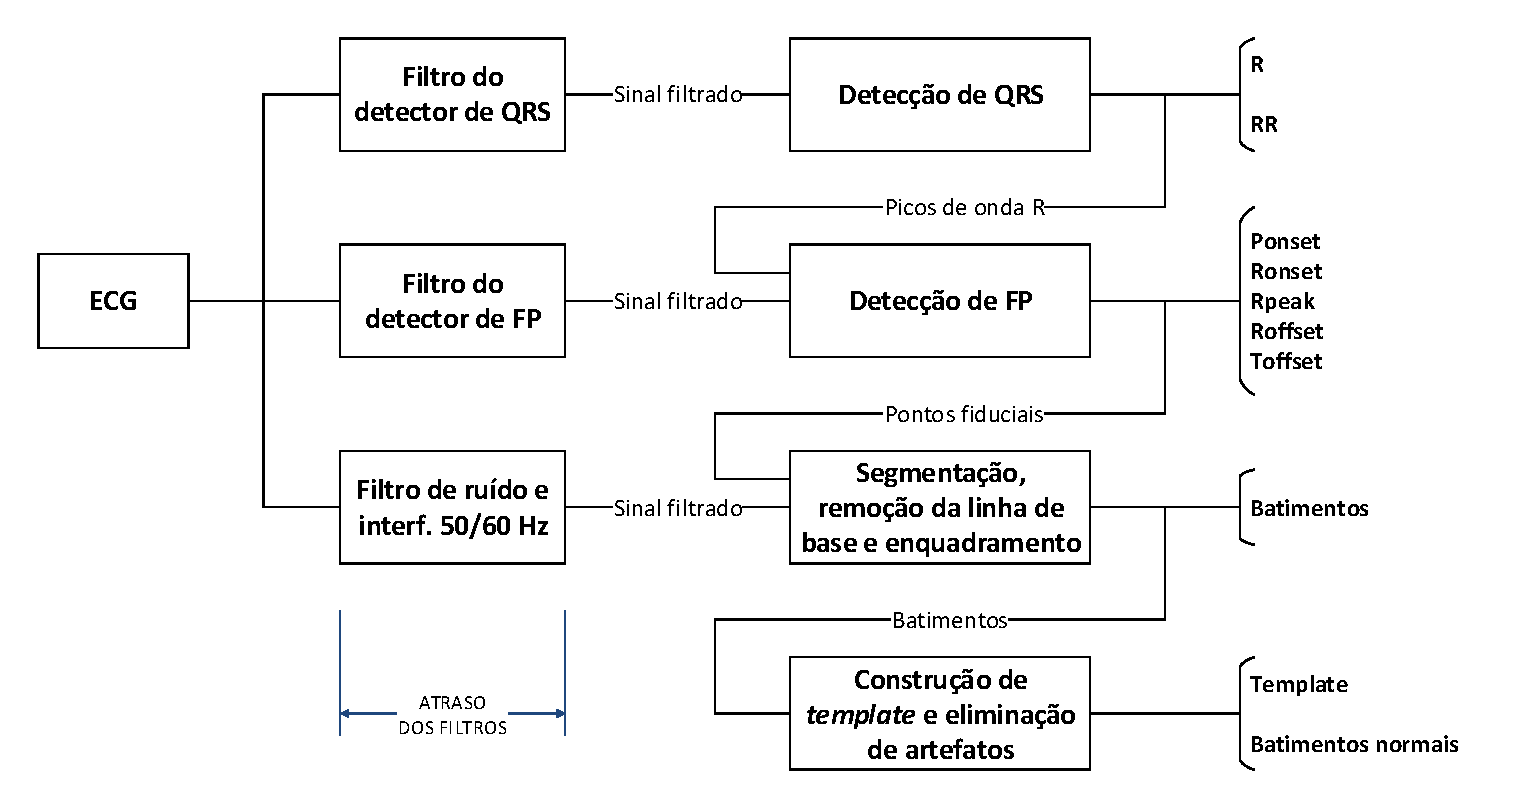
\includegraphics[width=450pt]{figures/chap6-preprocessing-diagram.pdf}
    \caption[Diagrama de blocos da estratégia de pré-processamento]{Diagrama de blocos da estratégia de pré-processamento. Produzida no Microsoft Visio.}
    \label{fig:preprocessdiag}
\end{figure}

O primeiro item de informação provém da detecção de QRS. O algoritmo utilizado para tal fim é aquele descrito por Pan e Tompkins \cite{Pan1985}. Este algoritmo é também descrito no livro de um dos autores \cite[pp. 245-262]{Tompkins1993} e avaliado em outro artigo \cite{Hamilton1986}. A escolha deste algoritmo segue a escolha feita por dois dos métodos de detecção de isquemia, o de Mohebbi e Moghadam e o de Gopalakrishnan et al., mas também se deve ao fato de que ele constitui uma técnica robusta e tradicional na área de processamento de sinais biomédicos.

Na prática, a lista R é desnecessária aos métodos de detecção de isquemia, pois, como veremos mais adiante, os batimentos são segmentados e embutidos num quadro (\emph{frame}) de tamanho pré-definido. Sendo este tamanho um número ímpar e estabelecendo que os batimentos dentro do quadro estejam centralizados no pico de onda R, tem-se que o pico está sempre no ponto central do quadro, dispensando o uso da lista na etapa de extração.

Esta lista serve, porém, para apuração do resultado dos métodos, em termos das métricas introduzidas no capítulo \ref{chap:chapter4}. Sabemos que as anotações do ECG fornecem a localização dos batimentos conforme auditada por especialistas e, portanto, se faz necessário para fins de avaliação conhecer a localização obtida pelo detector de QRS. Dadas duas listas de pontos, há um algoritmo que faz o casamento cruzado entre elas. Isto é, que combina batimentos de uma lista com os da outra contanto que estejam muito próximos temporalmente. Este algoritmo é apresentado na rotina \texttt{match\_qrs} (código-fonte \ref{lst:matchqrs}), escrita em código MATLAB.

O segundo item de informação não é simplesmente a diferença entre picos de onda R sucessivos, mas sim uma estimativa média do intervalo RR calculada a cada novo batimento. A estimativa tem portanto o efeito de ``suavizar'' a medida, eliminando variações demasiado abrutas de frequência cardíaca\footnote{a frequência cardíaca (em batimentos por minuto) pode ser obtida a partir do intervalo RR, pela expressão $\frac{60f_s}{RR}$, onde $f_s$ é a frequência de amostragem do conversor A/D}. A lista RR provém do mesmo algoritmo de detecção de QRS, sendo necessária por dois motivos: primeiro porque o método de Rocha et al. emprega uma técnica de determinação do ponto J (definido logo adiante) fazendo uso da medida de frequência cardíaca; segundo porque Gopalakrishnan et al. lançam mão do intervalo RR na sua etapa de extração.

O terceiro item advém de um algoritmo proposto por Yan Sun et al. \cite{Sun2005}. Originalmente, o procedimento faz a marcação dos seguintes pontos de interesse (ou \emph{fiducial points}):
\begin{description}
    \item[$\{P_{onset}, P_{peak}, P_{offset}\}$] pontos inicial, de pico e final da onda P;
    \item[$\{Q_{onset}, Q_{peak}, Q_{offset}\}$] pontos inicial, de pico e final da onda Q;
    \item[$\{R_{onset}, R_{peak}, R_{offset}\}$] pontos inicial, de pico e final da onda R;
    \item[$\{S_{onset}, S_{peak}, S_{offset}\}$] pontos inicial, de pico e final da onda S; e
    \item[$\{T_{onset}, T_{peak}, T_{offset}\}$] pontos inicial, de pico e final da onda T.
\end{description}
Contudo, apenas os pontos de início da onda P, os pontos da onda R e o ponto final da onda T são realmente necessários para os fins deste trabalho. $R_{onset}$ e $R_{offset}$ servem para realizar a busca de dois outros pontos de interesse: o isoelétrico e o $J$, definidos informalmente abaixo.
\begin{mydef}
    Ponto isoelétrico é o local designado para o batimento onde este apresenta amplitude de ``nível zero'' antes do início da onda R. Isto é, o ponto à esquerda de $R_{onset}$ que pode ser considerado como referência para a troca de polaridade das amplitudes do batimento cardíaco.
\end{mydef}
\begin{mydef}
    Ponto $J$ é o local designado para o batimento onde o seu ``traço'' se torna mais horizontal do que vertical, após o término da onda R. Isto é, o ponto à direita de $R_{offset}$ que pode ser considerado como início de um período de inatividade elétrica do coração.
\end{mydef}

O ponto isoelétrico (aqui, apelidado de $I$) e o ponto $J$ são obtidos por um algoritmo distinto, descrito por Daskalov em \cite{Daskalov1998}. A técnica em essência detecta as bordas do batimento cardíaco com auxílio da derivada de primeira ordem do sinal. Quem a sugere é Mohebbi e Moghadam, para uso na delimitação do segmento ST. Os mesmos pontos são necessários ao método de Rocha et al., por dois motivos: primeiro porque o ponto $I$ servirá de referência para a estimativa do desvio ST, medido como a diferença entre as amplitudes no ponto $J$ e naquele; segundo porque o ponto $J$ serve como separador dos segmentos utilizados na etapa de extração do método (rever seção \ref{sec:rocha}). Rocha et al., que sugerem o uso do algoritmo de Sun citado anteriormente, requerem os pontos inicial e final do batimento, $P_{onset}$ e $T_{offset}$, principalmente por dois motivos: para remoção da linha de base e para delimitação dos segmentos usados na etapa de extração. A identificação da linha de base é feita por uma aproximação polinomial envolvendo as bordas de cada batimento, daí a necessidade destes pontos.

No método de Mohebbi e Moghadam, a remoção da linha de base seria alcançada através de interpolação \emph{spline} cúbica, segundo um artigo de Badilini \cite{Badilini1991}. A técnica requer conhecimento apenas da localização dos picos de onda R e é de fácil implementação para o caso de trincas -- isto é, usando, além do batimento atual, o seu precedente e o sucessor. Contudo, num sistema de tempo-real, haverá necessidade de aguardar a detecção de um novo batimento cardíaco para que possa ser feita a interpolação para o batimento atual, o que incorre em um atraso equivalente a um batimento. No pior caso, o batimento seguinte pode nunca ser detectado. Ademais, a interpolação é mais precisa se se lançar mão das derivadas do sinal nas extremidades, implicando a necessidade de dois pontos adicionais (um antes do precedente e um depois do sucessor). Finalmente, a aproximação se deteriora à medida que a frequência cardíaca diminui, pois então o maior afastamento entre os pontos na interpolação prejudica o ajuste de amplitudes em torno do ponto central. Em virtude dessas desvantagens, neste trabalho foi escolhida a técnica anterior.

O quarto item de informação é constituído pelos próprios batimentos cardíacos, depois de segmentados, filtrados, sem linha de base e enquadrados num \emph{frame} de tamanho fixo. O tamanho do \emph{frame} foi estabelecido como $1,2$ vezes o número de amostras em $1$ segundo do sinal. De acordo com \cite{Clifford2006}, a duração de um ciclo cardíaco está entre 0,6 e 1 segundo. Dando uma margem de tolerância de $0,2$ segundos ao valor máximo, garante-se que a vasta maioria dos batimentos caibam no \emph{frame}. Caso o tamanho resultante seja um número par, o incrementa-se de 1 para que a condição previamente especificada seja satisfeita (pico de onda R no centro do emph{frame}).

A segmentação, portanto, consiste em delimitar o batimento cardíaco por seus pontos inicial e final, centralizá-lo pelo seu pico de onda R e enquadrá-lo no \emph{frame}. O enquadramento remove qualquer trecho que esteja fora do quadro, tanto à esquerda quanto à direita do centro, bem como preenche com zeros caso ``sobre'' espaço no quadro. A remoção da linha de base ocorre antes deste procedimento, porque utiliza a informação completa do sinal do batimento. Conforme sugerido por Rocha et al., a técnica para identificação da linha de base é adaptada de Wolf \cite{Wolf2004}, que faz a interpolação usando um polinômio de primeiro grau.

O quarto item corresponde ao \emph{template}, que é construído progressivamente ao longo da execução. O uso de \emph{template} se faz necessário para o método de Mohebbi e Moghadam, que o utiliza para extrair um modelo de segmento ST. Os autores também o requerem afim de eliminar artefatos que foram identificados erroneamente como batimento pelo detector QRS. A eliminação se dá por meio de uma medida de erro, neste caso a distância Euclideana, obtida pela norma da diferença entre os vetores que descrevem o template e o batimento avaliado. Aproveitando-se dessa exigência, incorporou-se um algoritmo iterativo de construção do \emph{template} à etapa de pré-processamento. Dessa forma, todos os métodos de detecção de isquemia se beneficiam da eliminação de artefatos, o que propicia uma comparação mais justa. Para o método de Mohebbi e Moghadam, que necessita de um \emph{template} explicitamente, toma-se então a versão de \emph{template} que ocorre depois de processados os primeiros 30 ciclos cardíacos.

A filtragem do sinal de ECG para remoção de ruído e interferência, conforme ilustra a figura \ref{fig:preprocessdiag}, é realizada em paralelo com a detecção de QRS e de FP. Essa filtragem se dá pela aplicação de dois filtros IIR: um passa-baixas de Butterworth seguindo a especificação dada por Rocha et al., para redução de ruído de alta-frequência; e um rejeita-faixas Chebyshev tipo I com banda de rejeição de 2 Hz, para eliminação da interferência da rede elétrica. O projeto desses filtros, diferentemente do projeto dos filtros da detecção QRS e FP, é feito de antemão por intermédio do MATLAB, para várias frequências de amostragem comuns em eletrocardiografia.

Uma decisão de projeto que merece menção é o fato de ter-se aberto mão da transformada discreta de Wigner-Ville. Este procedimento era requerido pelo método de Rocha et al. para a localização dos pontos $I$ e $J$. Entretanto, a implementação desta transformada em linguagem de programação tradicional não é trivial. Ela envolve o uso de variáveis complexas, da transformada de Fourier discreta (DFT) e da transformada de Hilbert, além de ser bastante custosa em termos de processamento. O uso de variáveis complexas significa que deve-se trabalhar com dois vetores em memória, um para a parte real e outro para a parte imaginária do sinal. O uso da transformada de Fourier implica que devemos selecionar e incorporar um algoritmo de FFT (\emph{Fast Fourier Transform}) ao ferramental do trabalho. A transformada de Hilbert, que, segundo os autores, é necessária para obtenção de um sinal analítico antes da aplicação da Wigner-Ville, parece ser tão cheia de peculiaridades que alguns professores a consideram matéria de pós-graduação. Esses fatores tornam a implementação mais complicada e demorada, não só pela complexidade mas porque todo código desenvolvido deve ser testado e validado. 

Há ainda o fato de que, dado um vetor de tamanho $n$, são necessários $n$ cálculos de DFT para obter a transformada de Wigner-Ville do vetor. Não bastasse isso, a matriz resultante deve passar por operações de valor absoluto e de soma, em que as linhas correspondentes a baixas frequências são superpostas para formar o vetor subjacente à busca dos pontos desejados. As duas últimas observações indicam que o procedimento exige bastante processamento. E de fato isso ocorre: fez-se uma tentativa de implementação usando a linguagem MATLAB (que possui funções prontas de DFT, Hilbert, manipulação de matrizes e de números complexos), e determinou-se que o tempo de processamento deste item perfazia mais da metade do tempo de extração de características do método.

Outra questão é que, nesta tentativa de implementação da transformada de Wigner-Ville, o resultado da identificação dos pontos $I$ e $J$ foi medíocre. O que ocorre é que os pontos de mínimo não são tão bem definidos e, muitas vezes, não existem dentro dos intervalos de busca (lembre-se de que os próprios autores não deixam claro os limites dos intervalos). Em virtude de todas estas considerações, decidiu-se não utilizar a transformada de Wigner-Ville para localização dos pontos $I$ e $J$. Em vez disso, reaproveitou-se a técnica utilizada por Mohebbi e Moghadam (aquela que faz uso de diferenciação e \emph{thresholding}).

\subsection*{Implementação}

A implementação aconteceu de três formas, cada uma em um momento diferente. Primeiro criou-se um ambiente de trabalho usando a ferramenta computacional MATLAB. Neste caso, diversas rotinas de tratamento dos sinais de ECG foram implementadas em código MATLAB, e serviram para testar e validar o funcionamento da estratégia adotada. Em seguida, criou-se códigos na linguagem C que realizam as mesmas tarefas de maneira equivalente, e estes foram validados pela comparação de seus resultados com aqueles obtidos usando o código MATLAB. Num terceiro momento, construiu-se um modelo de simulação em tempo real, usando a ferramenta Simulink do MATLAB. Nesta implementação, utilizou-se a linguagem C++, que oferece recursos de orientação a objetos e permite uma melhor organização do código-fonte.

O desenvolvimento em C e em C++ se deu através do próprio MATLAB, que oferece uma API (\emph{Application Programming Interface}) para uso e compilação de códigos C/C++ na sua plataforma. Não serão feitas aqui referências ao código em C nem C++, apenas ao código MATLAB. Além disso, devido ao tamanho do trabalho, somente algumas rotinas em MATLAB serão apresentadas, todas no apêndice \ref{app:matlab} desta monografia. Caso o leitor deseje visualizar o código completo, tanto em MATLAB quanto em C ou C++, refira-se ao seguinte link: \url{https://github.com/dsogari/tg-ecp-ufrgs}. Ali estará o repositório do trabalho desenvolvido disponível para \emph{download} gratuito. Este repositório será atualizado constantemente até a conclusão do trabalho, o que pode não coincidir com a entrega desta monografia.

Os sinais de ECG são os da base de dados ST-T da Sociedade Européia de Cardiologia \cite{Taddei1992}, obtidos a partir do \emph{website} PhysioBank.org da PhysioNet \cite{Goldberger2000}. A leitura dos arquivos da base foi realizada com auxílio do pacote de software WFDB, disponibilizado gratuitamente pelo mesmo \emph{site}. Na verdade, para facilitar o trabalho no MATLAB, criou-se algumas rotinas que encapsulam as chamadas do WFDB e produzem arquivos .mat contendo todas as informações de um ECG. Assim, para ler um arquivo de ECG basta carregar o .mat correspondente usando as funções nativas do MATLAB, que são bastante simples e eficientes.

Uma estrutura em MATLAB contém as amostras do sinal e outras informações a respeito deste, como a frequência de amostragem, o valor de referência e a resolução do conversor A/D, anotações, entre outras. Esta estrutura serve como entrada para a etapa de pré-processamento. A etapa começa pela filtragem do sinal de ECG, descrita em detalhes a seguir.

A filtragem para detecção de complexos QRS se dé pela função \texttt{qrs\_filter} (código \ref{lst:qrsfilter}). Esta função recebe como parâmetros as amplitudes do sinal de ECG e a frequência de amostragem, $f_s$. Ela retorna o sinal filtrado e o atraso total dos filtros, $d_{QRS}$. Os filtros deste procedimento são quatro: um passa-baixas de segunda ordem\footnote{\label{fnt:note1}esta ordem não diz respeito ao número de coeficientes do filtro, mas sim tem a ver com os coneitos apresentados no capítulo \ref{chap:chapter3}, no que tange à técnica de projeto de filtros FIR com coeficientes inteiros} com frequência de corte em aproximadamente 11 Hz; um passa-altas de primeira ordem\footnote{Ver nota de rodapé \ref{fnt:note1}}. com frequência de corte em aproximadamente 5 Hz; um diferenciador de 5 pontos; e um filtro de média-movel com largura aproximada de 150 ms.

A filtragem para detecção de pontos de interesse se dé pela função \texttt{fp\_filter} (código \ref{lst:fpfilter}). Esta função recebe como parâmetros as amplitudes do sinal de ECG, a frequência de amostragem e o atraso $d_{QRS}$. Ela retorna dois sinais, um que corresponde à derivada de primeira ordem do sinal de entrada suavizado e outro que é a derivada morfológica \cite{Sun2002} do sinal suavizado. Os filtros deste procedimento são quatro: um passa-baixas de segunda ordem\footnote{Ver nota de rodapé \ref{fnt:note1}} com frequência de corte em aproximadamente 11 Hz; um filtro de média-movel com largura de aproximadamente 50 ms; um diferenciador de dois pontos; e um filtro de média-movel com largura aproximada 150 ms.

A filtragem para remoção de ruído se dé pela função \texttt{noise\_filter} (código \ref{lst:noisefilter}). Esta função recebe como parâmetros as amplitudes do sinal de ECG, a frequência de amostragem, a frequência da rede elétrica, $f_m$, e novamente o atraso $d_{QRS}$. Ela retorna o sinal filtrado, isto é, sem ruído de alta frequência e sem interferência da rede elétrica. Há dois filtros neste procedimento: um passa-baixas de Butterworth de quarta ordem com frequência de corte em aproximadamente 40 Hz; e um rejeita-faixas de quarta ordem Chebyshev tipo I, com frequência central em $f_m$ e largura da banda de rejeição de aproximadamente 2 Hz.

Os atrasos das três filtragens seriam dados a grosso modo por: $d_{QRS} \approx 0.18f_s$, $d_{FP} \approx 0.09f_s$ e $d_{noise} \approx 0.01f_s$. Entretanto, deseja-se ``emparelhar'' os sinais filtrados. Isto é, fazer com que eles estejam na mesma linha de tempo após a filtragem. Isso facilita o trabalho dos detectores na etapa de pré-processamento. Sabendo que $d_{QRS}$ é o maior dos três atrasos, tem-se que as demais devem ser igualadas àquela. A equivalência de atrasos é alcançada pela introdução de filtros passa-tudo, com um atraso dado pela diferença entre $d_{QRS}$ e $d_{FP}$ ou entre $d_{QRS}$ e $d_{noise}$. Para uma frequência de amostragem de 250 Hz, que é aquela da base de dados utilizada, tem-se $d_{QRS} = 46.5$ amostras. Também vale dizer que a frequência da rede elétrica usada nos testes foi 50 Hz, uma vez que a base de dados é européia.

O próximo passo é detectar os batimentos. A função que realiza tal procedimento é \texttt{detect\_qrs} (código \ref{lst:detectqrs}). Ela recebe como parâmetros as amplitudes do sinal filtrado pelos filtros QRS e a taxa de amostragem. Ela retorna a localização aproximada dos picos de onda R e uma estimativa média dos intervalos RR. Existem cinco componentes principais no laço deste algoritmo: detecção de picos, atualização de \emph{thresholds}, determinação de complexos QRS, atualização de medidas de intervalo RR e busca de QRS em retrospecto (\emph{searchback}). Para cada pico detectado, verifica-se se a amplitude é maior que um \emph{threshold}. Se for, então o pico é candidato a ser de um complexo QRS. Medidas de nível de ruído e de sinal são atualizadas de acordo com a decisão tomada para o pico. O \emph{threshold} é computado em função desses níveis. Caso nenhum complexo QRS seja detectado dentro de um determinado período, a busca em retrospecto é ativada para recuperar um possível complexo perdido. A localização do pico do complexo, que quase sempre corresponde ao pico de onda R, não é identificada exatamente pelo algoritmo. O importante é saber que há um complexo QRS nos instantes próximos ao pico detectado no sinal filtrado. A localização exata no ECG é obtida pela detecção de pontos fiduciais, descrita a seguir.

A detecção de pontos fiduciais se dá pela função \texttt{detect\_fp} (código \ref{lst:detectfp}). Ela recebe como parâmetros os dois sinais filtrados pela filtragem FP e a lista R fornecida pelo detector QRS. Sua saída é uma lista com os pontos fiduciais correspondentes a cada item da lista R. A busca é dividida em três partes. Em primeiro lugar são detectados os pontos referentes à onda R ($R_{peak}$, $R_{onset}$ e $R_{offset}$). Em segundo lugar, tendo $R_{onset}$, detecta-se o pico e o início da onda P ($P_{peak}$ e $P_{onset}$). Lembre-se de que $P_{peak}$ não será necessário posteriormente, mas é imprescindível para a busca de $P_{onset}$. Por último, tendo $R_{offset}$, detecta-se o pico e o fim da onda T ($T_{peak}$ e $T_{offset}$). Novamente, $T_{peak}$ não será necessário para a etapa de extração, mas serve para encontrar $T_{offset}$. A busca é feita com ajuda de algumas rotinas especiais: \texttt{search\_peak\_abs}, \texttt{search\_first\_mark} e \texttt{search\_best\_mark}. Em particular, a busca dos picos ($R_{peak}$, $P_{peak}$ e $T_{peak}$) desconsidera a polaridade do sinal. Isto é, um pico negativo é identificado da mesma maneira que um pico positivo, utilizando a rotina \texttt{search\_peak\_abs}.

A segmentação dos batimentos pode agora ser realizada, pois tem-se as marcações $P_{onset}$ e $T_{offset}$. Também com base nestes pontos, pode-se encontrar um polinômio de primeiro grau que melhor se ajusta à reta que conecta ambos. Mais especificamente, toma-se uma média das amplitudes nos cinco pontos próximos a $P_{onset}$ e nos cinco pontos próximos a $T_{offset}$. Com as médias, calcula-se os parâmetros da reta que os liga. Em cada ponto do batimento, subtrai-se da amplitude original o valor da reta avaliado naquele ponto. Tem-se assim um batimento cuja linha de base é o próprio eixo horizontal de nível zero (ou isoelétrico). Após a remoção da linha de base, o batimento é enquadrado num \emph{frame}, da maneira como foi explicada no início desta seção. A função que realiza estes procedimentos é \texttt{extract\_beats} (código \ref{lst:extractbeats}), com suas rotinas auxiliares \texttt{polyfit\_baseline} e \texttt{frame\_beat}. Os parâmetros de entrada de \texttt{extract\_beats} são as amplitudes do sinal filtrado pelos filtros de ruído, a lista FP e a taxa de amostragem. Sua saída é composta pela lista de batimentos extraídos e uma nova lista FP cujos valores dizem respeito à localização dos pontos de interesse no \emph{frame} (e não mais no ECG).

Finalmente, toma lugar a construção de \emph{template} e a remoção de artefatos. Para tanto, é usada a função \texttt{build\_template} (código \ref{lst:buildtemplate}). Esta função recebe como parâmetro a lista de batimentos e uma constante que diz a taxa de adaptação do \emph{template}. Por exemplo, uma taxa de $R$ significa que as amplitudes do \emph{template} obedecem à regra $T_i[n] = T_{i-1}[n] + R^{-1}\left(B_i[n] - T_{i-1}[n]\right), 0 \leq n \leq N-1$, com $N$ igual ao tamanho do \emph{frame} dos batimentos. Esta é a equação de recorrência de um filtro de média-móvel exponencial com constante de decaimento igual a $1/R$. No entanto, o \emph{template} só é atualizado se a diferença, $E$, entre o \emph{template} e o batimento atual for menor que um \emph{threshold}, $C$. Este \emph{threshold} é calculado pela mesma relação recursiva: $C_i = C_{i-1} + R^{-1}\left(E_i - C_{i-1}\right)$. O erro $E_i$ é a medida de diferença na i-ésima iteração, dada pela distância Euclideana: $E_i = \|B_i - T_i\|$. Na verdade, dois valores de \emph{threshold} são mantidos, um que equivale a 3 vezes o valor do erro médio e o outro, a 4 vezes o mesmo valor. Assim, se o erro na iteração atual for menor que o primeiro \emph{threshold}, então o batimento é considerado muito bom e tanto o \emph{template} quanto o \emph{threshold} são atualizados. Senão, se o erro estiver acima do segundo \emph{threshold}, então o batimento é considerado como artefato e descartado. Se o erro cair no intervalo entre os dois \emph{thresholds}, o batimento é considerado bom e mantido sem que haja alteração de \emph{template} ou de \emph{threshold}.


\section{Projeto da extração de características}

\subsection*{Método de Rocha et al.}
A extração de características do método de Rocha começa pela identificação do ponto $J$ através da técnica de Pang \cite{Pang2005}. A função que realiza este procedimento é \texttt{pang\_jpoint}. Ela recebe como parâmetro os intervalos RR e retorna a localização do ponto $J$ de acordo com o intervalo em que se encontra a frequência cardíaca, conforme mostra a tabela \ref{tab:pangpoints}.

\begin{table}[ht!]
    \centering
    \begin{tabular}{cc}
    \toprule
    Frequência cardíaca (em BPM) & Ponto de medida\\
    \midrule
    $<100$        & $R+120$ ms\\
    $100-110$  & $R+112$ ms\\
    $110-120$  & $R+104$ ms\\
    $>120$       & $R+100$ ms\\
    \bottomrule
\end{tabular}
    \caption[Localização do ponto $J$ determinada com base na frequência cardíaca]{Localização do ponto $J$ determinada com base na frequência cardíaca.}
    \label{tab:pangpoints}
\end{table}

Em seguida, o algoritmo de bordas é empregado para a busca do ponto isoelétrico e também para uma nova estimativa do ponto $J$. A função \texttt{edge\_detection} (código \ref{lst:edgedetection}), que recebe como parâmetros o sinal do batimento, pontos de início e fim, além de um \emph{threshold}, faz a busca do ponto desejado no intervalo, retornando este como saída. A busca do ponto $I$ se dá pela aplicação da função no intervalo à esquerda de $R_{peak}$, enquanto a busca de $J$ se dá no intervalo à direita de $R_{peak}$.

Com estes pontos, obtêm-se uma medida do desvio de segmento ST, dado pela diferença entre as amplitudes do batimento nos pontos $J$ e aquela avaliada no ponto $I$. Essas duas medidas são as primeiras a compor o conjunto de características do método de Rocha et al.

O próximo passo é seccionar o batimento em dois segmentos: um contendo o complexo QRS e outro contendo a onda T. O primeiro segmento vai do ponto $I$ até o ponto $J$, enquanto o segundo vai deste até o ponto final do batimento ($T_{offset}$). Cada um destes segmentos é então reamostrado para um sinal de 64 amostras. A função do MATLAB para reamostragem é \texttt{resample}. Ela recebe como parâmetros o sinal que se deseja reamostrar, um fator de interpolação $p$ e um fator de dizimação $q$, retornando um sinal de largura $\lceil\frac{p}{q}\rceil$ vezes a largura original. Internamente, essa função faz o projeto de um filtro passa-baixas FIR, necessário ao algoritmo de reamostragem.

Na implementação em C da reamostragem, foi usada a técnica de projeto de filtros por truncagem da resposta ideal, conforme vista no capítulo \ref{chap:chapter3}. O filtro projetado possui as seguintes especificações: largura da região de transição de 2 Hz, frequência de corte em $\frac{\pi}{\max\left(p,q\right)}$ radianos e uso da janela Hamming (que apresenta atenuação média de 41 dB na banda de rejeição). Note que o projeto é refeito a cada nova chamada de reamostragem, pois a especificação depende do tamanho do sinal original.

Os segmentos devidamente reamostrados servem como operando no produto matricial que fornece os coeficientes da expansão em funções de Hermite, sendo o outro operando a matriz discutida no capítulo \ref{chap:chapter5} para o método de Rocha et al. Há uma matriz para o primeiro segmento e outra para o segundo segmento, cada qual com seu fator de dilatação (5 e 8, para ser exato). Ambas possuem 6 linhas e 64 colunas, de modo que o produto com o vetor coluna contendo as 64 amostras do segmento correspondente resulta nos coeficientes desejados.

Portanto, ao final da extração do método de Rocha et al., obtêm-se um conjunto de 14 características, quais sejam: duas medidas de desvio de segmento ST; seis coeficientes da expansão de Hermite do primeiro segmento; e seis coeficientes da expansão do segundo segmento. A função responsável pelo garimpo de todos estes itens é \texttt{rocha\_features} (código \ref{lst:rochafeatures}), auxiliada pelas rotinas \texttt{pang\_jpoints}, \texttt{rocha\_ijpoints}, \texttt{rocha\_stdev}, \texttt{rocha\_segments} e \texttt{rocha\_hermite} (códigos \ref{lst:pangjpoints}, \ref{lst:rochaijpoints}, \ref{lst:rochastdev}, \ref{lst:rochasegments} e \ref{lst:rochahermite} respectivamente).

\subsection*{Método de Mohebbi e Moghadam}
A etapa de extraçao do método de Mohebbi e Moghadam começa com a localização do ponto $J$, pelo mesmo procedimento já mencionado, o da função \texttt{edge\_detection}. Depois, extrai-se o segmento ST, que inicia no ponto $J$ e se estende por 160 ms (ou 40 amostras, numa frequência de amostragem de 250 Hz). O segmento é reamostrado pra 20 amostras e sua diferença com o segmento ST do \emph{template} é obtida por uma simples operação de subtração.

Note-se que o ponto $J$ e o segmento ST do \emph{template} são extraídos apenas uma vez, tão logo o \emph{template} se faça presente. A versao de \emph{template} utilizda é aquela computada após o 30\ordm batimento. A função que executa estes procedimentos é \texttt{mohebbi\_features} (código \ref{lst:mohebbifeatures}), suportada pelas rotinas auxiliares \texttt{mohebb\_ijpoints}, \texttt{mohebb\_isegments} e \texttt{mohebb\_istdiff} (códigos \ref{lst:mohebbijpoints}, \ref{lst:mohebbisegments} e \ref{lst:mohebbistdiff}, respectivamente).

\subsection*{Método de Gopalakrishnan et al.}
A extração do método de Gopalakrishnan et al. é bastante simples. Primeiro, um segmento é extraído contendo todo o batimento. Ele está centralizado no pico de onda R (ou o centro do \emph{frame}) e possui largura igual ao intervalo RR correspondente ao batimento em questão. Subsequentemente, a função de reamostragem é aplicada para produzir um sinal de tamanho fixo igual a 250 amostras. 

Finalmente, ocorre o produto matricial entre a matriz de funções discretas de Hermite (ver capítulo \ref{chap:chapter3}), com 50 linhas e 250 colunas, e o vetor coluna com as 250 amostras do batimento. O resultado é um conjunto de 50 coeficientes, que compõem o conjunto de caracteristicas do método. A função que realiza estes procedimentos é \texttt{gopalak\_features} (código \ref{lst:gopalakfeatures}), juntamente com as rotinas auxiliares \texttt{gopalak\_segments} e \texttt{gopalak\_hermite} (códigos \ref{lst:gopalaksegments} e \ref{lst:gopalakhermite}, respectivamente).

\section{Projeto da classificação}

Para a etapa de classificação, cada autor sugere uma estrutura diferente de redes neurais, bem como procedimentos distintos de treinamento das mesmas. As tabelas \ref{tab:nnspecs} e \ref{tab:trainspecs} mostram os diversos aspectos dos três esquemas de classificação propostos.

\begin{table}[ht!]
    \centering
    \begin{tabular}{p{4cm}p{3.8cm}p{3.8cm}p{3.8cm}}
    \toprule
    \backslashbox{Item}{Método} & Rocha et al. & Mohebbi e Moghadam & Gopalakrishnan et al.\\ 
    \midrule
    Função de transferência   & tangente sigmóide & log-sigmóide & tangente sigmóide\\
    Função de normalização    & não especificado & não especificado & não especificado\\
    N\ordm de entradas        & 14 & 20 & 50\\
    N\ordm de saídas          & 1 & 1 & 2\\
    Intervalo da saída        & [-1,1] & [0,1] & [-1,1]\\
    N\ordm de camadas ocultas & 2 & 1 & 1\\
    N\ordm de neurônios       & depende da derivação & 20 & não especificado\\
    N\ordm de redes           & 2 & 1 & 5\\
    \bottomrule
\end{tabular}
    \caption[Especificações da estrutura das redes neurais segundo cada autor]{Especificações da estrutura das redes neurais segundo cada autor.}
    \label{tab:nnspecs}
\end{table}

\begin{table}[ht!]
    \centering
    \begin{tabular}{p{4cm}p{3.8cm}p{3.8cm}p{3.8cm}}
    \toprule
    \backslashbox{Item}{Método} & Rocha et al. & Mohebbi e Moghadam & Gopalakrishnan et al.\\ 
    \midrule
    Função de treinamento     & Levenberg-Marquardt (\texttt{trainlm}) & \emph{Backpropagation} adaptativo (\texttt{traingdx}) & Gradiente conjugado (\texttt{trainscg})\\
    Característica utilizada  & ST & ST & ST e T\\
    Proporção de ocorrência   & não especificado & 0.169 & não especificado\\
    Registros utilizados      & conferir tabela \ref{tab:selection} & conferir tabela \ref{tab:selection} & não especificado\\
    Divisão do conjunto para \emph{cross-validation} & não especificado & não especificado & não especificado\\
    N\ordm de amostras & depende da derivação & 18047 & 236\\
    Considera derivações separadamente & sim & não & não\\
    \bottomrule
\end{tabular}
    \caption[Especificações do esquema de treinamento segundo cada autor]{Especificações do esquema de treinamento segundo cada autor.}
    \label{tab:trainspecs}
\end{table}

\begin{table}[ht!]
    \centering
    \begin{tabular}{lp{5cm}p{6cm}}
    \toprule
    \backslashbox{Derivação}{Método} & Rocha et al. (descartados) & Mohebbi e Moghadam (utilizados)\\ 
    \midrule
    D3    & -- & --\\
    MLI   & e0207 & --\\
    MLIII & e0109, e0121, e0609, e0613 & e0103, e0105, e0113, e0119, e0147\\
    V1    & e0403 & --\\
    V2    & e0415 e0603 & --\\
    V3    & -- & --\\
    V4    & e0119 e0161 & e0103, e0105, e0113, e0119, e0147\\
    V5    & e0207, e0213, e0303, e0405 & --\\
    \bottomrule
\end{tabular}
    \caption[Seleção de registros da base pelos métodos]{Seleção de registros da base pelos métodos.}
    \label{tab:selection}
\end{table}

Assim como na etapa de pré-processamento, isso gera um problema prático: a implementação fica difícil e propensa a erros, pois a quantidade de código a ser escrito, mantido e testado é maior. Há novamente aqui uma motivação para criar um código único, que sirva para todos os métodos. Não apenas essa abordagem tende a tornar mais justa a comparação entre os métodos, mas facilita a implementação e encurta o tempo de desenvolvimento, do qual se carece. A solução então é combinar as diversas escolhas dos autores e encontrar uma combinação boa e conveniente para o esquema de classificação final. A seguir são descritas as escolhas feitas e o porquê de cada uma.

\begin{itemize}
    \item Algoritmo de treinamento \texttt{trainlm}: é o padrão do MATLAB; usado pelo método de Rocha et al.; é geralmente o mais rápido a convergir, segundo a documentação do MATLAB.
    \item Função de transferência tangente sigmóide (\texttt{tansig}): usado por dois dos métodos.
    \item Função de normalização \texttt{mapstd} (média 0 e desvio padrão 1): segundo colegas de trabalho, é a mais comumente utilizada.
    \item Divisão aleatória dos dados na proporção 75/15/15: como nenhum dos autores explicita a sua escolha para fins de \emph{cross-validation}, será utilizada a divisão padrão do MATLAB, que é de 75\% para treinamento, 15\% para validação e 15\% para teste (de modo aleatório).
    \item Saída única: o treinamento é mais rápido do que com 2 ou mais saídas (verificado experimentalmente); quando as saídas dizem respeito a informações independentes (caso do terceiro método), as chances de sucesso são maiores usando duas redes separadas.
    \item 2 camadas ocultas com número aleatório de neurônios: intuitivamente, 2 camadas devem fornecer resultado melhor do que uma; um número fixo de neurônios durante o treinamento seria interessante apenas se se comprovasse que um número é melhor que outro.
    \item Saída indica presença ou ausência da característica: tanto a característica de desvio de segmento ST quanto a da onda T na verdade são decompostas em outras 2, que são a elevação ou depressão do segmento ST e a elevação ou depressão da onda T. As possíveis classes então seriam aquelas dadas na tabela \ref{tab:nnclasses}. No entanto, considerando as redes com saída única, tem-se um número elevado de redes a serem treinadas. Portanto, decidiu-se utilizar a presença ou ausência de cada característica separadamente, mas sem distinguir entre elevação ou depressão. O resultado são duas redes: uma indicando presença/ausência de desnivelamento ST e a outra, presença/ausência de desnivelamento da onda T.
    \item Uso das proporções de ocorrência da base: apenas um dos autores sugere a composição do conjunto de dados usando uma proporção específica de batimentos normais \emph{versus} isquêmicos. Assim, decidiu-se levantar estatísticas sobre a proporção de ocorrência de cada característica na base, e estas servirão como referência na seleção dos dados. Mais detalhes serão discutidos na seção \ref{sec:tests}.
    \item Uma rede para cada derivação: na implementação das etapas de processamento anteriores, percebeu-se que as formas de onda -- e, consequentemente, as características extraídas -- de diferentes derivações são bastante díspares; Rocha et al. também apontam este fato e dizem ser a separação uma boa escolha para melhorar os resultados. Como a base possui ECGs de 8 derivações diferentes, tem-se um total de 8 redes para cada método.
    \item Seleção dos dados de acordo com resultados de ECGs individuais: num primeiro momento, os conjuntos de dados continham exatamente os mesmos registros de ECG sugeridos por cada autor (ver tabela \ref{tab:selection}). Contudo, os resultados obtidos foram pífios. Ao fazer o treinamento das redes para cada registro individualmente, notou-se que muitos dos resultados eram bons, enquanto outros estavam aquém do esperado. Concluiu-se que os vetores de características da fase de extração para estes últimos não representavam corretamente os batimentos detectados. Porquanto não há uma maneira simples e automatizada de avaliar a consistência dos dados extraídos, optou-se por utilizar os próprios resultados individuais como critério de seleção. Mais detalhes serão discutidos na seção \ref{sec:tests}.
\end{itemize}

\begin{table}[ht!]
    \centering
    \begin{tabular}{lccc}
    \toprule
    \backslashbox{ST}{T} & Normal & Elevado & Deprimido\\
    \midrule
    Normal    & $C_{11}$ & $C_{12}$ & $C_{13}$ \\
    Elevado   & $C_{21}$ & $C_{22}$ & $C_{23}$ \\
    Deprimido & $C_{31}$ & $C_{32}$ & $C_{33}$ \\
    \bottomrule
\end{tabular}
    \caption[Possíveis classes do procedimento de classificação]{Possíveis classes do procedimento de classificação.}
    \label{tab:nnclasses}
\end{table}

Há que se mencionar que os dois primeiros métodos não utilizam as características de desvio da onda T no seu procedimento de classificação. Rocha et al. deixam claro esta escolha, enquanto Mohebbi e Moghadam não explicitam a sua. Acredita-se que estes tenham utilizado apenas o desvio de segmento ST, pois é com base neste segmento que o vetor de características do método é extraído. Gopalakrishnan et al., por outro lado, dizem claramente que utilizam as duas características (ST e T). Assim, tem-se um total de (2 métodos $\times$ 1 característica $+$ 1 método $\times$ 2 características) $\times$ 8 derivações $=$ 32 redes neurais a serem treinadas para uma dada seleção de conjuntos de dados.

A classe a que pertence um batimento é dada pela condição $y>0$, onde $y$ é um valor real entre -1 e 1, correspondente à saída de uma rede neural. A condição satisfeita indica que a característica observada está presente, e o contrário é verdadeiro ($y\leq 0 \rightarrow$ característica ausente). Para julgar se um batimento é isquêmico, basta perguntar se $y>0$ nos dois primeiros métodos, ou perguntar se $y_1>0$ || $y_2>0$ no método de Gopalakrishnan et al., pois este tem duas redes (ST e T).

Outra questão importante é manter a proporção de ocorrência das características na população quando se faz uma seleção dos dados de treinamento das redes neurais. Este é o conceito de \textbf{estratificação}. Se existir muito mais batimentos com a característica observada do que realmente existe na população, a probabilidade de que a rede produza muitos falsos positivos é grande. Portanto, deve-se procurar manter a proporção original da população (que seria a base de ECGs).

Alguns códigos da etapa de classificação em MATLAB são apresentados no apêndice \ref{app:matlabclass}. As rotinas principais de treinamento são \texttt{train\_network} e \texttt{train\_networks} (códigos \ref{lst:trainnetwork} e \ref{lst:trainnetworks}); as rotinas \texttt{generate\_datasets} e \texttt{generate\_lead\_dataset} (códigos \ref{lst:generatedatasets} e \ref{lst:generateleaddataset}) são relativas à seleção de dados para composição dos conjuntos de treinamento, a ser discutida na próxima seção.

\section{Projeto dos testes}
\label{sec:tests}

Conforme discutido anteriormente, fez-se necessário o levantamento das proporções de ocorrência das características de isquemia (ST e T) na base de ECGs. Já foi mencionado que a base contém registros de 8 derivações diferentes. Cada uma destas apresenta o seu percentual de ocorrência tanto no quesito ST como no T. A título de exemplo, as figuras \ref{fig:mlistclass} e \ref{fig:v4stclass} mostram num gráfico do tipo ``pizza'' os percentuais encontrados para a característica ST nas derivações MLI e V4, respectivamente. Da mesma forma, as figuras \ref{fig:mlitclass} e \ref{fig:v4tclass} ilustram a distribuição de ocorrência da característica T. O mesmo estudo foi feito para as demais derivações, de modo a possuir todos os percentuais de ocorrência necessários à construção dos conjuntos de dados.

\begin{figure}[ht]
    \centering
    \begin{subfigure}[b]{.4\textwidth}
        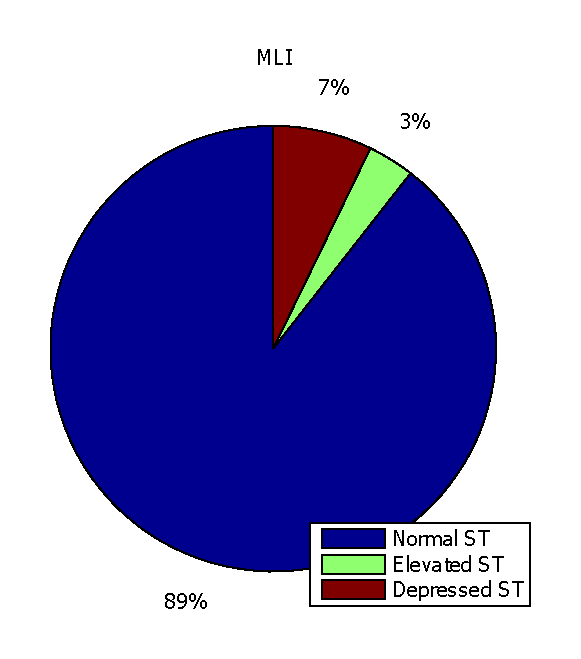
\includegraphics[width=\textwidth]{figures/chap6-mli-st-class-dist.pdf}
        \caption{Derivação MLI}
        \label{fig:mlistclass}
    \end{subfigure}
    \begin{subfigure}[b]{.4\textwidth}
        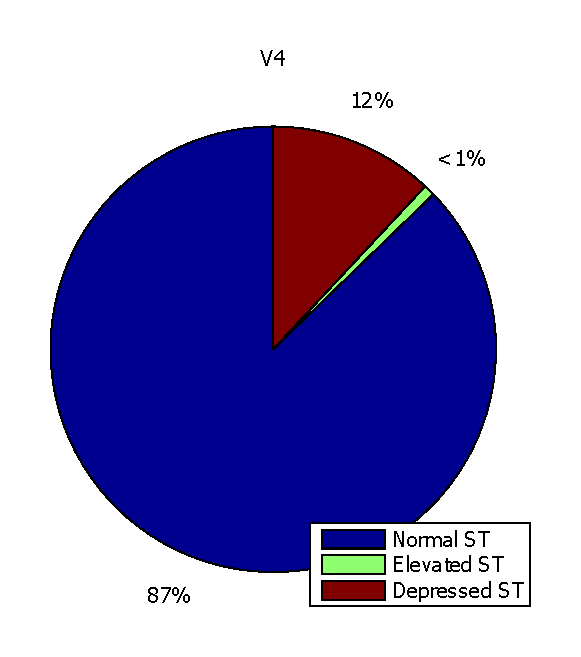
\includegraphics[width=\textwidth]{figures/chap6-v4-st-class-dist.pdf}
        \caption{Derivação V4}
        \label{fig:v4stclass}
    \end{subfigure}
    \caption[Gráficos de distribuição da característica ST na base]{Gráficos de distribuição da característica ST na base. Produzidos no MATLAB.}
\end{figure}

\begin{figure}[ht]
    \centering
    \begin{subfigure}[b]{.4\textwidth}
        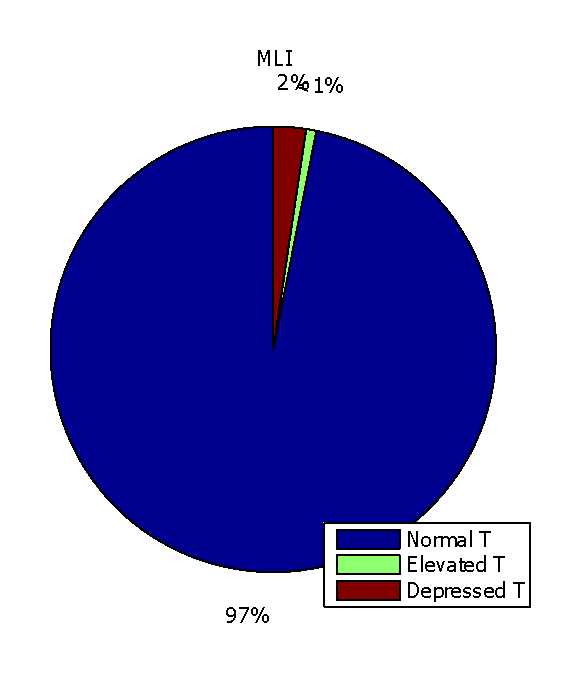
\includegraphics[width=\textwidth]{figures/chap6-mli-t-class-dist.pdf}
        \caption{Derivação MLI}
        \label{fig:mlitclass}
    \end{subfigure}
    \begin{subfigure}[b]{.4\textwidth}
        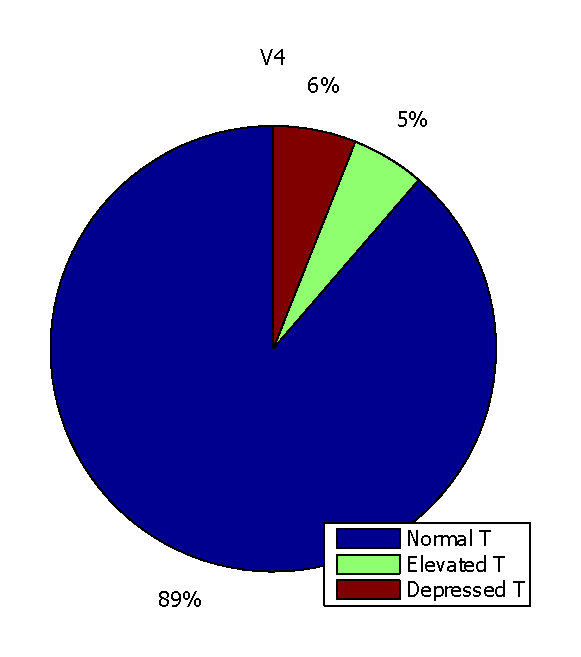
\includegraphics[width=\textwidth]{figures/chap6-v4-t-class-dist.pdf}
        \caption{Derivação V4}
        \label{fig:v4tclass}
    \end{subfigure}
    \caption[Gráficos de distribuição da característica T na base]{Gráficos de distribuição da característica T na base. Produzidos no MATLAB.}
\end{figure}

Foi discutido também que a proposta original dos autores para seleção dos dados não rendeu resultados satisfatórios. Portanto, far-se-á um estudo para determinar quais os registros de ECG da base que mais prejudicam o desempenho geral. Quer-se então criar 5 configurações diferentes de seleção de conjuntos de dados para treinamento:

\begin{description}
    \item[Configuração 1] proposta original dos autores, mantendo inclusive o número de batimentos.
    \item[Configuração 2] proposta criada com base no desempenho obtido com redes individuais.
    \item[Configuração 3] da configuração anterior, faz-se uma junção (ou \emph{merger}) entre as listas dos diferentes métodos, privilegiando a decisão da maioria.
    \item[Configuração 4] mesma seleção da configuração 3, só que restringindo o número de batimentos selecionados (mas mantendo a estratificação).
    \item[Configuração 5] conjunto completo extraído da base, sem descarte
\end{description}

Nas configurações 1 e 2, cada método possui sua própria seleção de registros e número de batimentos, enquanto nas demais a seleção se mantém igual para os três métodos. Um resumo desta estratégia pode ser visualizado na figura \ref{fig:selection}. Na figura, os canais 0 ou 1 dizem respeito a um dos vetores de amostras de ECG contidos num registro da base (todos contêm 2 canais).

\begin{figure}[ht]
    \centering
    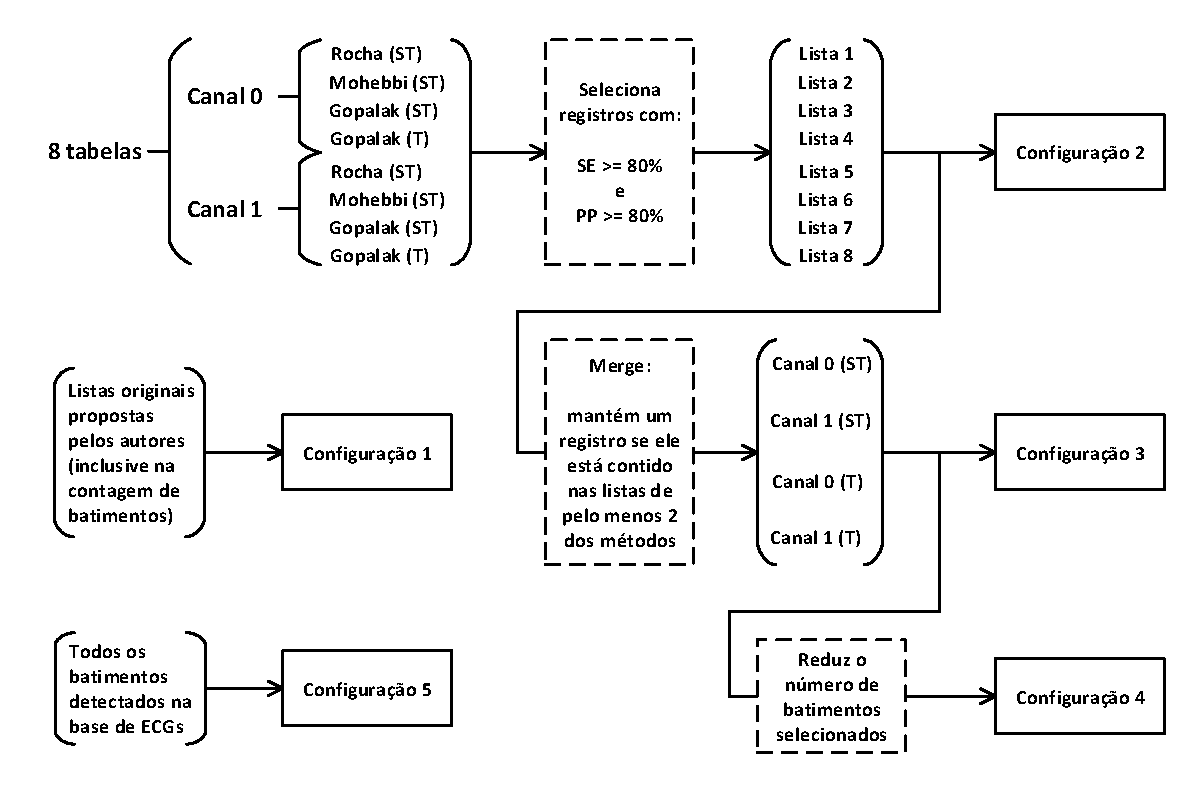
\includegraphics[width=470pt]{figures/chap6-selection-scheme.pdf}
    \caption[Esquema de seleção de conjuntos de dados]{Esquema de seleção de conjuntos de dados para o treinamento das redes neurais. Produzido no Microsoft Visio.}
    \label{fig:selection}
\end{figure}

Com esta estratégia, haverá 5 configurações $\times$ 32 $=$ 160 redes neurais a serem treinadas. Também seria necessário apresentar, no capítulo seguinte, 8 tabelas de resultados individuais e 20 tabelas de resultados coletivos, pois são 5 configurações $\times$ 4 instâncias de treinamento e teste (Rocha et al. para ST, Mohebbi e Moghadam para ST e Gopalakrishnan et al. para ST e T). A fim de não poluir o espaço do próximo capítulo com diversas tabelas, será feita uma análise um pouco diferente: primeiro será apresentada uma tabela de exemplo contendo a primeira instância de teste; em seguida serão mostradas tabelas contendo o resultado médio de todos os registros para o caso individual e de todas as derivações para o caso coletivo. Dessa forma, haverá cerca de 9 ou 10 tabelas concisas, contendo as informações relevantes para uma análise comparativa de confiabilidade dos métodos.

\section{Resumo}

Neste capítulo foram apresentados os projetos das etapas de pré-processamento, extração e classificação, bem como um projeto dos testes a serem realizados para comparação de desempenho dos métodos.

Primeiramente, na etapa de pré-processamento, viu-se que há a quatro procedimentos principais: a detecção de complexos QRS; a detecção de pontos de interesse; a segmentação e eliminação da linha de base; e por último a construção de \emph{template} e eliminação de artefatos. Os três primeiros são precedidos, cada qual, por uma filtragem do sinal de ECG. A filtragem realça características que são importantes ao procedimento correspondente. O resultado desta etapa são os batimentos cardíacos, os intervalos RR, os pontos de interesse em cada batimento e também um \emph{template} de batimento normal. Vale lembrar que os procedimentos desta etapa são os mesmos para todos os métodos de detecção de isquemia.

Na etapa de extração, os batimentos submetem-se às técnicas de processamento propostas pelos autores dos métodos, embora com algumas modificações. No método de Rocha et al., o desvio de segmento ST é calculado com base nos pontos $I$ e $J$, e os coeficientes de Hermite são obtidos após uma nova segmentação do batimento em duas partes, com subsequente reamostragem para limitar o número de amostras. O vetor de características deste método contém 14 valores. No método de Mohebbi e Moghadam, o ponto $J$ serve como referência para obtenção do segmento ST, que também é reamostrado. O vetor de características deste método tem tamanho 20 e corresponde à diferença entre o segmento ST testado e o do \emph{template}. Por fim, o método de Gopalakrishnan et al. utiliza o intervalo RR para limitar ainda mais o batimento dentro do quadro e fazer a reamostragem para 250 amostras. Subsequentemente, produz-se 50 coeficientes na expansão de Hermite, compondo estes o vetor de características do método.

A etapa de classificação merece atenção especial, pois cada autor sugere uma estratégia diferente. Com o intuito de concluir o trabalho em tempo hábil, optou-se por uniformizar o esquema de treinamento e classificação. As redes possuirão saída única, indicando presença ou ausência de uma determinada característica de isquemia. Apenas o método de Gopalakrishnan et al. utiliza-se de duas características, viz. o desvio de segmento ST e a inversão da onda T, enquanto os demais utilizam apenas aquela relativa ao segmento ST. Dessa forma, tem-se 4 grupos de treinamento, cada qual com 8 redes neurais (uma para cada derivação de ECG), totalizando 32 redes a serem treinadas. Porém, conforme foi visto na seção \ref{sec:tests}, serão criadas 5 configurações diferentes de seleção dos conjuntos de dados de treinamento, fazendo com que o total suba para 160 redes.

Ainda na seção \ref{sec:tests}, abordou-se a questão da estratificação dos dados, que está relacionada ao percentual de ocorrência de cada característica na população de ECGs. Uma levantamento foi feito para descobrir as diversas proporções de ocorrência tanto do desvio de segmento ST quanto do desvio da onda T.

Este capítulo constitui a parte mais importante do trabalho, pois foi aqui que as diversas escolhas de projeto e de implementação foram descritas e devidamente justificadas.